% JEL-Article.tex for AEA last revised 22 June 2011
\documentclass[AER]{AEA}

% The mathtime package uses a Times font instead of Computer Modern.
% Uncomment the line below if you wish to use the mathtime package:
%\usepackage[cmbold]{mathtime}
% Note that miktex, by default, configures the mathtime package to use commercial fonts
% which you may not have. If you would like to use mathtime but you are seeing error
% messages about missing fonts (mtex.pfb, mtsy.pfb, or rmtmi.pfb) then please see
% the technical support document at http://www.aeaweb.org/templates/technical_support.pdf
% for instructions on fixing this problem.

% Note: you may use either harvard or natbib (but not both) to provide a wider
% variety of citation commands than latex supports natively. See below.

% Uncomment the next line to use the natbib package with bibtex 
\usepackage{natbib}
\usepackage{hyperref} 
\usepackage{bbm}
\usepackage{enumerate}
\usepackage[shortlabels]{enumitem}
\usepackage{graphicx}

% Other settings for numbering theorems
\let\proof\relax
\let\endproof\relax
\usepackage{amsthm}
\newtheorem{theorem}{Theorem}[section]
\newtheorem{lemma}[theorem]{Lemma}
\newtheorem{conj}[theorem]{Conjecture}

% Uncomment the next line to use the harvard package with bibtex
%\usepackage[abbr]{harvard}

% This command determines the leading (vertical space between lines) in draft mode
% with 1.5 corresponding to "double" spacing.
\draftSpacing{1.5}

\begin{document}

\title{Inequality and Ex-Post Fairness in Rationing Mechanisms}
\shortTitle{(Exploration of Open Questions)}
\author{Eric Tang\thanks{%
Thanks to Mohammad Akbarpour, Matthew Gentzkow and Paul Milgrom for thoughtful discussions on and support for these ideas.}}
\date{\today}
\pubMonth{Month}
\pubYear{Year}
\pubVolume{Vol}
\pubIssue{Issue}
\JEL{}
\Keywords{}

\begin{abstract}
    In market design settings where agents have differing marginal utilities for money, the socially optimal mechanism may involve rationing agents out of the market. However, less work has studied the optimality of rationing in settings with risk-aversion or wealth effects, such as labor markets. In this work, we analyze the optimal single-price mechanism on the seller side of a market for an indivisible good. We generalize the welfare maximization problem in this setting when agents have general preferences for money, and analyze optimal prices for several distributions using numerical simulation. In our simulation results, we find that rationing can still be optimal when agents have slightly concave preferences, but concave preferences do bring the welfare-maximizing price closer to the competitive price.
\end{abstract}

\maketitle

\section{Main Question}

Recent years have seen a proliferation of work on fair allocation in market design, by modeling agents with varying utility functions, and designing allocation and pricing mechanisms to address inequality in these markets. This work spans the fields of computer science, operations research, and economics. Among others, this work includes that of \cite{babaioff-2019}, \cite{akbarpour-2020} and \cite{budish-2011}. These are also natural extensions of the broader work on matching markets in the computer science literature, such as that of \cite{alaei-2017}.

One work we focus on is \cite{dworczak-2020}, who models a two-sided market with buyers and sellers who have differing marginal utilities for a good and for money. This can be viewed as a way to more highly value monetary transfers to agents with high marginal utility for money, who often have lower incomes. They then derive optimal mechanisms to maximize total welfare under these two-sided markets. In cases of significant same-side inequality, the optimal mechanism they derive is a randomized (rationing) mechanism, in which some agents can only trade with a given probability. As the authors point out, this randomization can in practice be harmful to poorer individuals, who may have less tolerance for uncertainty. This raises several possible approaches for addressing these harms in practice.

Our first approach is as follows: we will derive optimal mechanisms in the altered model where agents have risk-averse preferences. This extends the linear utility functions of agents which are assumed in the current model. To extend this to risk-averse settings, we will parametrize agents' utility functions for money as one of a family of concave functions, where this parameter differs across agents. We can then use similar techniques to the original work of \cite{dworczak-2020} to derive the optimal mechanism, by determining optimal mechanisms for the seller side, for the buyer side, and finally for the market as a whole. We hypothesize that maximizing social welfare for agents with risk-averse (concave) utility functions will result in optimal mechanisms favoring wedge mechanisms over rationing mechanisms.

We will begin our exploration of this first approach by simulating our existing optimal mechanisms in a setting with agents who have risk-averse utility functions. This will suggest in what cases the optimal mechanisms for risk-neutral agents differ from the optimal mechanisms for risk-averse agents. We will continue our exploration by deriving utility-maximizing mechanisms in the risk-neutral case. As milestones along the way, we will derive mechanisms in the simpler settings which the paper initially lays out: with one price on each side of the market, then up to two prices on each side of the market, and finally, with any possible allocation and pricing mechanism.

Another approach is to change our model of the good. Can we improve on ex-post fairness when the good is divisible? In such a market, the designer would not be constrained solely to either giving each buyer a good or not giving them a good, but could distribute the good more evenly among these buyers. In such a market, instead of randomly choosing which of the rationed buyers are granted access to the market, the market designer might allocate smaller quantities of the good among those buyers, (hopefully) improving ex-post fairness. One might also hope to optimize such market designs based on measures of ex-post fairness, such as the minimal ex-post utility of all agents in the resulting market outcome. Examples of real-world market designs for divisible goods which are motivated by equity could include the provisioning of medical care, or rationing for limited supplies of food.

Section \ref{sec:background-redist} reviews recent literature in market design for redistribution which is relevant to the proposed work. Section \ref{sec:ideas} lays out other open questions related to the two proposed question above, which could be used as extensions to this work.

\section{Background: Redistribution through Markets}
\label{sec:background-redist}

Price regulations, such as rent control and minimum wage laws, typically face tradeoffs between reducing inequality and maintaining efficient outcomes. In an age of dramatic inequality, it is critical to design markets with equity in mind.

Early work exploring this balance includes \cite{weitzman-1977}, who asks whether competitive prices or rationing in a one-commodity market is more effective at ensuring agents with the highest need receive the good. Weitzman focuses primarily on goods which are deemed a societal need, potentially including housing, food, or medical care. As in actual marketplaces, agents have both differing incomes and differing needs for the good. Intuitively, if income distribution is relatively egalitarian and agents' needs vary widely, then competitive prices better identifies those agents with greater need. On the other hand, if income inequality is high compared to the dispersion in need for the good, rationing is more effective.

Formally, \cite{weitzman-1977} reach these results by parametrizing agents' demand functions according to $\lambda$ and $\epsilon$, where $\lambda$ represents the agent's marginal value for money (falls as income rises) and $\epsilon$ represents the agent's need for the good. Critically, these types are unobservable by the market designer, a problem which will arise again in later work as well.

Weitzman now considers two possible rules for allocating a fixed quantity of the good to each agent. Under competitive prices, the market designer sets a price to ensure market clearing. Under pure rationing, the market designer equally divides the good between all agents. Note that \cite{dworczak-2020} build on this model by, among other improvements, considering more nuanced rationing schemes that allocate to a subset of agents or impose multiple price levels. Weitzman then may compute a loss for each method in meeting actual need, and compare the two schemes' outcomes based on the prior distributions of $\lambda$ and $\epsilon$ in the populace. This formalizes the intuition of when rationing or competitive prices better satisfy needs in the market.

\cite{dworczak-2020} characterize the Pareto frontier of this tradeoff by framing price regulation as a market design problem, with buyers and sellers seeking to buy an indivisible good. They frame the Pareto frontier as determining the welfare-maximizing solution when agents have different valuations for money and for the good. (Roughly speaking, the valuation for money falls with an agent's wealth). They find that when there is significant inequality between buyers and sellers, optimal price controls take the form of a ``tax" which charges buyers a lower price than that of sellers, then transfers the surplus to the poorer side of the market. When there is significant inequality between agents on one side of the market, price controls take a more complex form but may still be optimal.

The key obstacle which \cite{dworczak-2020} overcomes, as was faced by earlier models such as Weitzman (1977), is that the market designer does not perfectly identify agents' needs, and hence setting a price at which the commodity is rationed helps to identify these needs.

One interesting novelty of the \cite{dworczak-2020} model is their use of agents' differing marginal values for money, instead of the more standard approach of giving agents different Pareto weights to construct the Pareto frontier. The authors show that these two formulations are actually equivalent. Intuitively, an agent having a higher marginal utility for money is akin to a market designer placing greater weight on the money they are given in the final allocation. They show that agents' actions are fully characterized by their rate of substitution between the good and money.

The bulk of the paper describes the optimal mechanisms to address cross-side inequality (between sellers and buyers) and same-side inequality (between agents on the same side of the market). The paper discusses applications in markets for kidney exchange (rather, the one market which runs in Iran), which is generally an example of same-side inequality among sellers. It also discusses applications in the housing rental market, which is generally an example of cross-side inequality.

% Possible TODO: Could better-explain the mechanisms used, and the case studies examined.

The paper raises several interesting extensions. Most immediately, the model only studies an indivisible good without wealth effects. Both of these modeling assumptions could be extended. The model also neglects possible aftermarkets of trade between agents, which could be explicitly modeled. Finally, the rationing mechanism used to address same-side inequality is randomized; work on designing non-random mechanisms could be fruitful. It would also be interesting to find real-world examples where this randomization impacts participant behavior in measurable ways.

% Interesting! In the Redistributive Allocation paper, the authors mention that they are planning on applying the work to vaccines in an upcoming paper.

\cite{akbarpour-2020} approach the problem slightly differently, as one in which a market designer is alllocating a public good of heterogeneous quality to buyers, and additionally deciding on the price. Also notable about the \cite{akbarpour-2020} model is that it weights the valuation of generating revenue with its own Pareto weight, reflecting the potential uses of that generated revenue. Finally, the work also introduces observable types which the market designer can condition on: one can think of these as observable demographics which are partially informative about a buyer's need or their marginal utility for money. \cite{akbarpour-2020} is meant to be more ``applied'' than its predecessor, giving policymakers more concrete recommendations, and Piotr Dworczak has mentioned in a seminar that the authors are applying this paper's results to a model for vaccine distribution.

\section{Potential Research Ideas}
\label{sec:ideas}

\begin{enumerate}
    \item Recent years have seen a proliferation of work on fair allocation in market design to address inequality, spanning the theoretical computer science and economics literature. One example is \cite{akbarpour-2020}, whose proposed mechanism maximizes expected net welfare given buyers and sellers with differing marginal utilities for a good and for money. This can be viewed as a way to more highly weight the utilities of those agents with low marginal utility for money, who often have lower incomes. In cases of significant same-side inequality, the optimal mechanism they derive is a randomized (rationing) mechanism, in which some agents can only trade with a given probability.

    As the authors point out, this randomization can in practice be harmful to poorer individuals, who may have less tolerance for uncertainty. This raises several possible approaches addressing these harms in practice.
    
    One approach is as follows: can we explicitly model agents as having risk-averse preferences, and continue to derive the optimal mechanism under these circumstances? This should entail extending the linear agent preferences which are assumed in the current model. For example, one could imagine analyzing this mechanism for agents whose marginal utilities for money fall into a family of decreasing functions, parametrized by a parameter which differs across agents.
    
    A second approach could be to consider divisible goods. For example, instead of randomly choosing which of the rationed buyers are granted access to the market, the market designer might allocate smaller quantities of the good among those buyers. One might also hope to optimize such market designs based on measures of ex-post fairness, such as the minimal ex-post utility of all agents in the resulting market outcome. Examples of real-world market designs for divisible goods which are motivated by equity could include the provisioning of medical care, or rationing for limited supplies of food.

    Other questions on the theme of ex-post fairness include the following (these are less concrete). Can we model the harm to poorer agents in this model that results from randomization? Can we develop a mechanism that ``trades off'' efficiency for less randomization? Could these answers change if the good is divisible? If this game is repeated, can we explicitly choose which agents are rationed to reduce ex-post unfairness? Are there established metrics of ex-post fairness which we can use to evaluate this metric?

    \item For a fairly technical extension, in the accompanying seminar talk for \cite{akbarpour-2020}, Piotr Dworczak notes that their work only considers the case when there are a finite number of different label groups $i$ (the observable characteristics), but their work could likely be extended to the continuous case (when Pareto weights are continuous). This could be an interesting technical extension, but I'm not sure what the real-world analogue of interest would be here.
    
    \item Very interesting: taking \cite{akbarpour-2020} as a departure point, what if one incorporates externalities of the good's distribution into our optimization? It seems that many public provisioning systems are also partially motivated by positive externalities. One motivating question here is the distribution of vaccines, but one could imagine similar positive externalities in public provision of housing and education.
    
    \item \cite{akbarpour-2020} value revenue generation by giving revenue its own Pareto weight, representing the value of revenue to the market designer. This is quite important; in many congestion pricing models, for example, how the revenue is spent almost completely determines whether a congestion toll is progressive or regressive. Can we model revenue redistribution in this model more explicitly?

    \item In a larger vein, it remains to model the markets of \cite{dworczak-2020} in conjunction with much of the literature on taxation and macroeconomic redistribution. What might happen if we have a government tax collector who can directly observe incomes, and another market designer (the subject of \cite{akbarpour-2020}) who cannot? How do their optimal mechanisms interact?
    
    \item \cite{pathak-2020} develop results in the theory of reserves, when there are various categories of a good in reserve, and agents are eligible for each reserve based on what eligibility categories they fall into. What if goods in the reserves are heterogeneous in quality, and agents have preferences over the quality of goods? This extension would be analogous to the way that \cite{akbarpour-2020} extended Condorelli (2013), expanding the work to include items of heterogeneous quality. That said, I'm not quite sure what the real-world analogy would be here. The original model of \cite{pathak-2020} focused on medical supplies such as vaccines and ventilators; I'm not sure how salient preferences over quality are in this domain.
\end{enumerate}

% TODO: Define low inequality from the Dworczak paper, so you can cite it later.

\section{Risk-Averse Agents}

\section{Economic Intuition}

As a motivating example to consider the limitations of \cite{dworczak-2020}, consider an example in labor markets, where agents may be quite risk-averse about the income they receive. In our case, consider a group of taxi drivers (sellers) queued up and hoping to sell rides to a set of passengers (buyers). Sellers in this case may be risk-averse, as they may prefer a lower guaranteed income (a transfer) to an uncertain probability of a higher reward (being rationed into the market and making a sale). Thus with risk-averse preferences for money, we might expect that the optimal mechanism is more likely to utilize a competitive price accompanied by lump-sum transfers, instead of rationing.

As rationing is generally used more often in the seller side, we may naturally be more concerned with risk-averse preferences for sellers. As in the case of sellers entering a market to earn their income, this suggests that we should first concern ourselves with agents' risk-averse preferences for money. For example, a taxi driver may be less risk-averse with respect to the time it takes to accept a ride, but may be fairly risk-averse with regards to the income they accumulate in a given day.

\section{Framework}

In our modeling framework, we preserve much of the notation from \cite{dworczak-2020}. We continue to consider an indivisible good $K$, a divisible good $M$ representing money, a unit mass of prospective sellers, and a mass $\mu$ of prospective buyers. Our main departure will be to model risk-aversion of agents over money.

\subsection{Preferences}

Our first departure is our modeling of the preference of agents. Here we wish to capture a world in which buyers and sellers are risk-averse over money, though not necessarily over the good $K$. However, we would also like to maintain the notion that agents have varying marginal utilities for both money and the good $K$. Again, let $v^K$ denote an agent's marginal utility for good $K$ and let $v^M$ denote an agent's marginal utility for $M$. 

We then can characterize possible preferences for agents by utility functions of the form

$$
u(x^K, x^M; v^K, v^M) = v^K x^K + w(x^M; v^M)
$$

where $w$ denotes agents' utility for money, parametrized by their marginal utility for money $v^M$. To model our risk-aversion scenario, this utility function $w$ should satisfy three criteria. First, it should be concave (representing risk aversion). Second, the agent's marginal utility for money when they have no money should be $v^M$. Third, agents' utilities for a given amount of money should be increasing in their marginal valuation $v^M$. We formalize these conditions as

\begin{enumerate}[(i)]
    \item $w'' > 0$ (concavity)
    \item $w'(0; v^M) = v^M$ (marginal utility)
    \item For all $x^M$ and all $v^{M'} > v^M$, $w(x^M; v^{M'}) > w(x^M; v^M)$ (increasing in $v^M$)
\end{enumerate}

In this work, we will specify the utility function for money as an exponential function, which allows us to interpolate between highly concave and mildly concave functions. For a risk-averse agent receiving quantities $x^V$ and $x^M$ of the good and of money, respectively, we may define their utility as

$$
u(x^K, x^M; v^K, v^M) =  v^K x^K + (v^M x^M + 1)^k
$$

for some $k \in (0,1)$. Note here that our chosen utility for money, $w(x^M; v^M) = (v^M x^M+1)^k$ satisfies our three desired criteria. Furthemore, $k$ lets us select more concave functions at lower values of $k$, and nearly linear functions for higher values of $k$. \footnote{Other specifications for $w$ are possible and satisfy our criteria, such as $w(x^M; v^M) = \log(v^M x^M + 1)$, but here we focus on our exponential specification.}

% TODO: Flesh this out to find a class of possible functions w so that we can interpolate between "very concave" functions and "nearly linear" functions w. This may entail, for some given w, taking some parameter k which shifts and interpolates w as necessary to get the result we want.

\section{Optimality on the Seller Side}

We now move to analyzing the optimal mechanism on the seller side, for a fixed quantity $Q$ of the good that the designer would like to purchase, and an existing revenue $R$ that they have.

\subsection{Economic Intuition}
\label{sec:economic-intuition}

Turning again to the three factors that influence the market designer in choosing a price $p_s$, we may consider again the effects of raising the price $p_s$. To review, the three effects of raising the price are

\begin{enumerate}[(a)]
    \item [-] A decrease in allocative efficiency, since we now may be allocating to agents with a lower marginal rate of substitution. 
    \item [-] The market designer must spend more to acquire $Q$ items, reducing the amount of the lump-sum transfer $R - p_SQ$.
    \item [+] Sellers who are rationed into the market receive a higher price for their sale.
\end{enumerate}

In comparison to the case of linear utilities, in this risk-averse scenario, we may find that agents prefer a higher lump-sum transfer to a higher price when they sell their good. This is because the lump-sum transfer is guaranteed to all agents, while agents may be risk-averse about their chance of being rationed into the market in (c).

% TODO: When the good is very valuable, we may really prefer a rationing solution?

\subsection{Maximization Problem}

The next complication is that since utility in money is non-linear, we can no longer solely characterize agents' utilities using their marginal rate of substitution between the good and money.

Second, the original work of \cite{dworczak-2020} separates the objective maximization into two components: the expected change in utility from transactions for sellers who are able to sell their good, and the expected additional utility from any lump sum to the sellers. However, since our preferences for money are now non-linear, we must now separate our objective maximization into components based on which agents are receiving each transfer. Concretely, we have three categories of sellers: those who are willing to sell and do sell, those who are willing to sell but cannot sell, and those who do not wish to sell.

First, to determine the relative proportion of each group of sellers, we must determine the quantity of sellers who are willing to sell at a price $p_S$. As utilities are non-linear, sellers' decision to trade also depends on the amount of the lump-sum payment $R - p_S Q$. We denote this quantity of sellers by $\tau$. This quantity is then

$$
\tau = \int_{\underline{v}^K, \underline{v}^M}^{\overline{v}^K, \overline{v}^M} \mathbbm{1}[w(p_s + R - p_SQ; v^M) \ge w(R - p_S Q ; v^M) + v^K] dF(v^K, v^M)
$$

For sellers who are able to sell their good, these agents have none of the good, receive the price $p_s$, and further receive a lump-sum transfer of $R - p_s Q$. Thus the contribution of these sellers is

\begin{equation}
    \frac{Q}{\tau} \int_{\underline{v}^K, \underline{v}^M}^{\overline{v}^K, \overline{v}^M} \mathbbm{1}[w(p_s + R - p_SQ; v^M) \ge w(R - p_S Q ; v^M) + v^K] w(p_s + R - p_SQ; v^M) dF(v^K, v^M)
\end{equation}

On the other hand, sellers who wish to sell their good but are rationed out of the market receive only the good and the lump sum transfer. Thus the contribution of these sellers is

\begin{equation}
    \frac{\tau - Q}{\tau} \int_{\underline{v}^K, \underline{v}^M}^{\overline{v}^K, \overline{v}^M} \mathbbm{1}[w(R - p_SQ; v^M) \ge w(R - p_S Q ; v^M) + v^K] (v^K + w(R - p_SQ; v^M)) dF(v^K, v^M)
\end{equation}

Finally, sellers who do not wish to sell receive only the good and the lump sum transfer as well, making the contribution of a unit of these sellers

\begin{equation}
    \int_{\underline{v}^K, \underline{v}^M}^{\overline{v}^K, \overline{v}^M} \mathbbm{1}[w(R - p_SQ; v^M) \le w(R - p_S Q ; v^M) + v^K] (v^K + w(R - p_SQ; v^M)) dF(v^K, v^M)
\end{equation}

Thus our complete maximization objective is

\begin{equation}
    \begin{split}
        & \frac{Q}{\tau} \int_{\underline{v}^K, \underline{v}^M}^{\overline{v}^K, \overline{v}^M} \mathbbm{1}[w(p_s + R - p_SQ; v^M) \ge w(R - p_S Q ; v^M) + v^K] w(p_s + R - p_SQ; v^M) dF(v^K, v^M) \\
        & + \frac{\tau - Q}{\tau} \int_{\underline{v}^K, \underline{v}^M}^{\overline{v}^K, \overline{v}^M} \mathbbm{1}[w(R - p_SQ; v^M) \ge w(R - p_S Q ; v^M) + v^K] (v^K + w(R - p_SQ; v^M)) dF(v^K, v^M) \\
        & + \int_{\underline{v}^K, \underline{v}^M}^{\overline{v}^K, \overline{v}^M} \mathbbm{1}[w(R - p_SQ; v^M) \le w(R - p_S Q ; v^M) + v^K] (v^K + w(R - p_SQ; v^M)) dF(v^K, v^M)
    \end{split}
\end{equation}

For a fixed revenue $R$, quantity $Q$, and valuation distribution $F$, we aim to select the $p_S$ which maximizes this welfare objective.

\section{Numerical Analysis}

We are particularly interested in how the gap between the competitive price and welfare-maximizing price changes as agents' preferences become more risk-averse. In our setting, this means analyzing how these two prices change as $k$ moves from $1$ (perfectly linear, non-risk-averse preferences) towards $0$ (more concave preferences).

% Tag the intuition section with a label to cite here.
Based on our intuition described above, we expect that in settings where the competitive price is optimal with linear utilities for money, the competitive price should still be optimal when agents have risk-averse preferences. Second, we expect that in settings where rationing is optimal with linear utilities for money, the optimal price should shift closer to the competitive price as agents' preferences become more concave. In these settings, the question most of interest to us is whether our results are robust to the introduction of slight concavity. That is, for values of $k$ near $1$, it may be that the competitive price is always optimal. Such a result would substantially weaken the theoretical case for the use of price controls and rationing on the seller side, even in cases of high inequality.

Thankfully for the earlier literature, our numerical simulation results suggest that rationing can still be optimal even in settings with concave preferences.\footnote{Code for our numerical simulations can be found at https://github.com/Etang21/redistribution-report-284. }

% TODO: Update the following citation to refer to an equation which you define above.
Figure \ref{k-vs-prices-inequality-low} displays a setting in which inequality is low, in the sense of \cite{dworczak-2020}. In this setting, when agents' utilities for wealth are linear, the welfare-maximizing price is the competitive price. Figure \ref{k-vs-prices-inequality-low} shows that the welfare-maximizing and competitive prices still coincide when agents have risk-averse preferences.

\begin{figure}
    \label{k-vs-prices-inequality-low}
    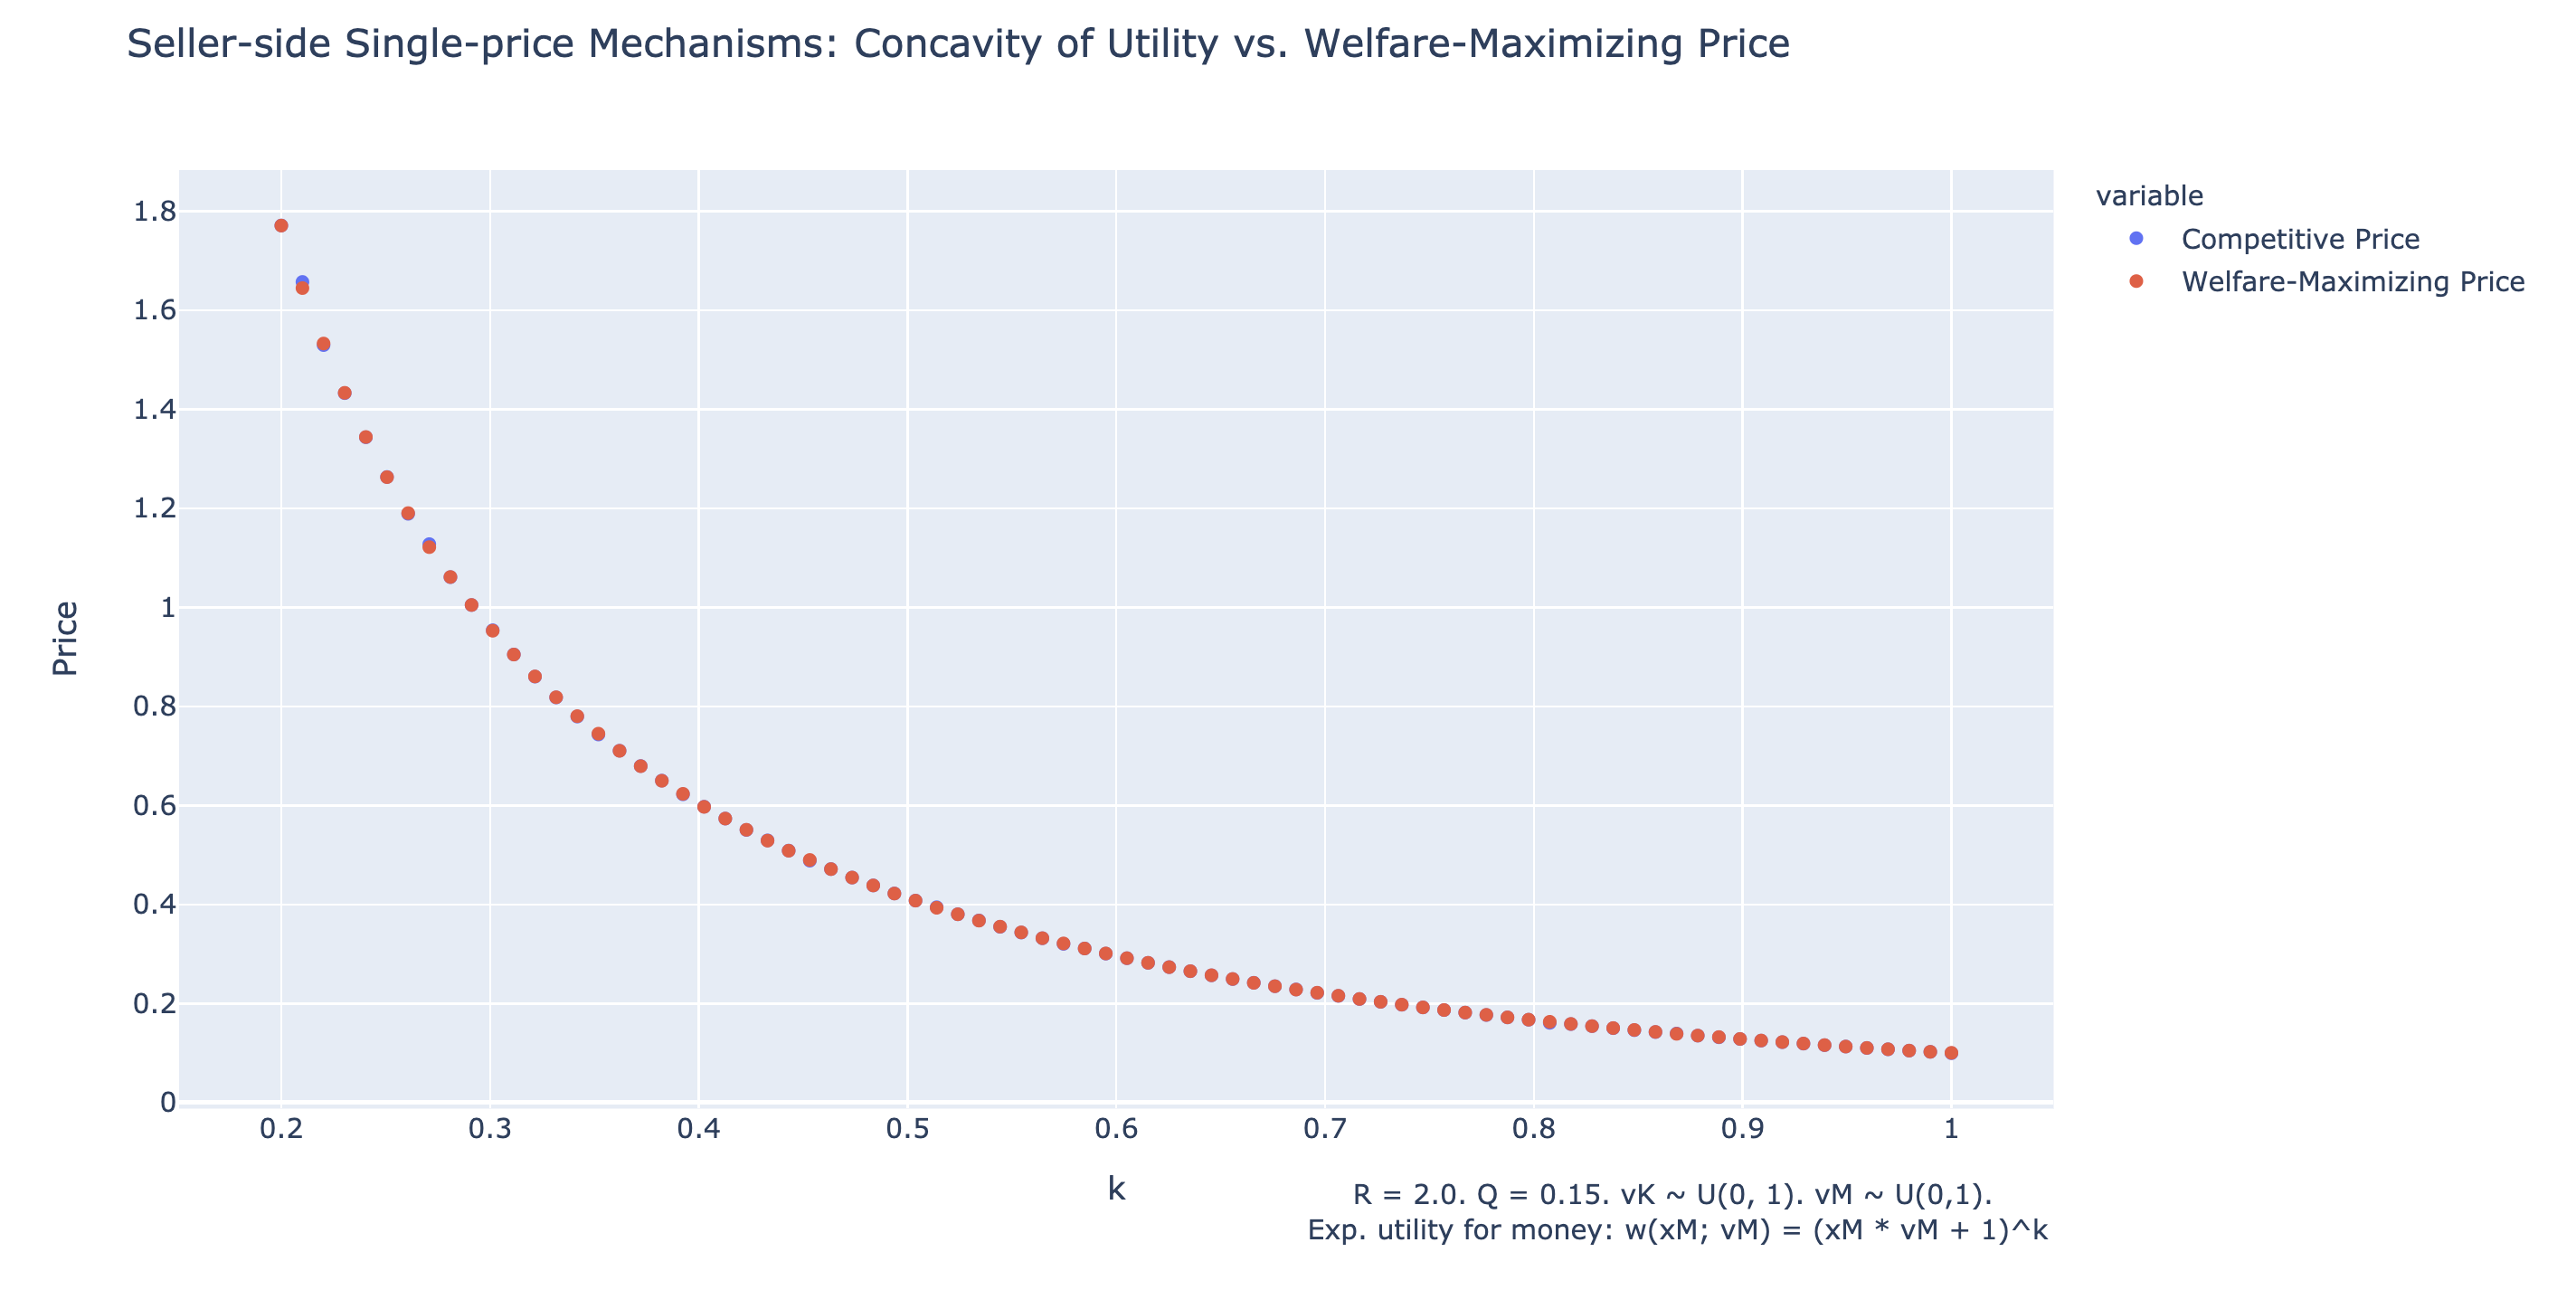
\includegraphics[width=\textwidth]{figures/k-vs-prices-inequality-low.png}
    \caption{Concavity of Utility (k) vs. Competitive Price and Welfare-Maximizing Price. Low-inequality setting.}
\end{figure}

Figure \ref{k-vs-prices-inequality-high} displays a setting in which inequality is high. In particular, we consider a setting where agents marginal utilities for the good are distributed as $v^K \sim U(0,1)$ and their marginal utilities for money are distributed as $v^M \sim \textrm{Pareto}(1/3)$. In this setting, when agents have linear utilities for money, the optimal mechanism is a single price above the competitive price, which results in rationing. In our numerical simulation, we find that when preferences are slightly concave, the optimal mechanism still utilizes rationing. When preferences are very concave, however, the optimal price coincides with the competitive price.

\begin{figure}
    \label{k-vs-prices-inequality-high}
    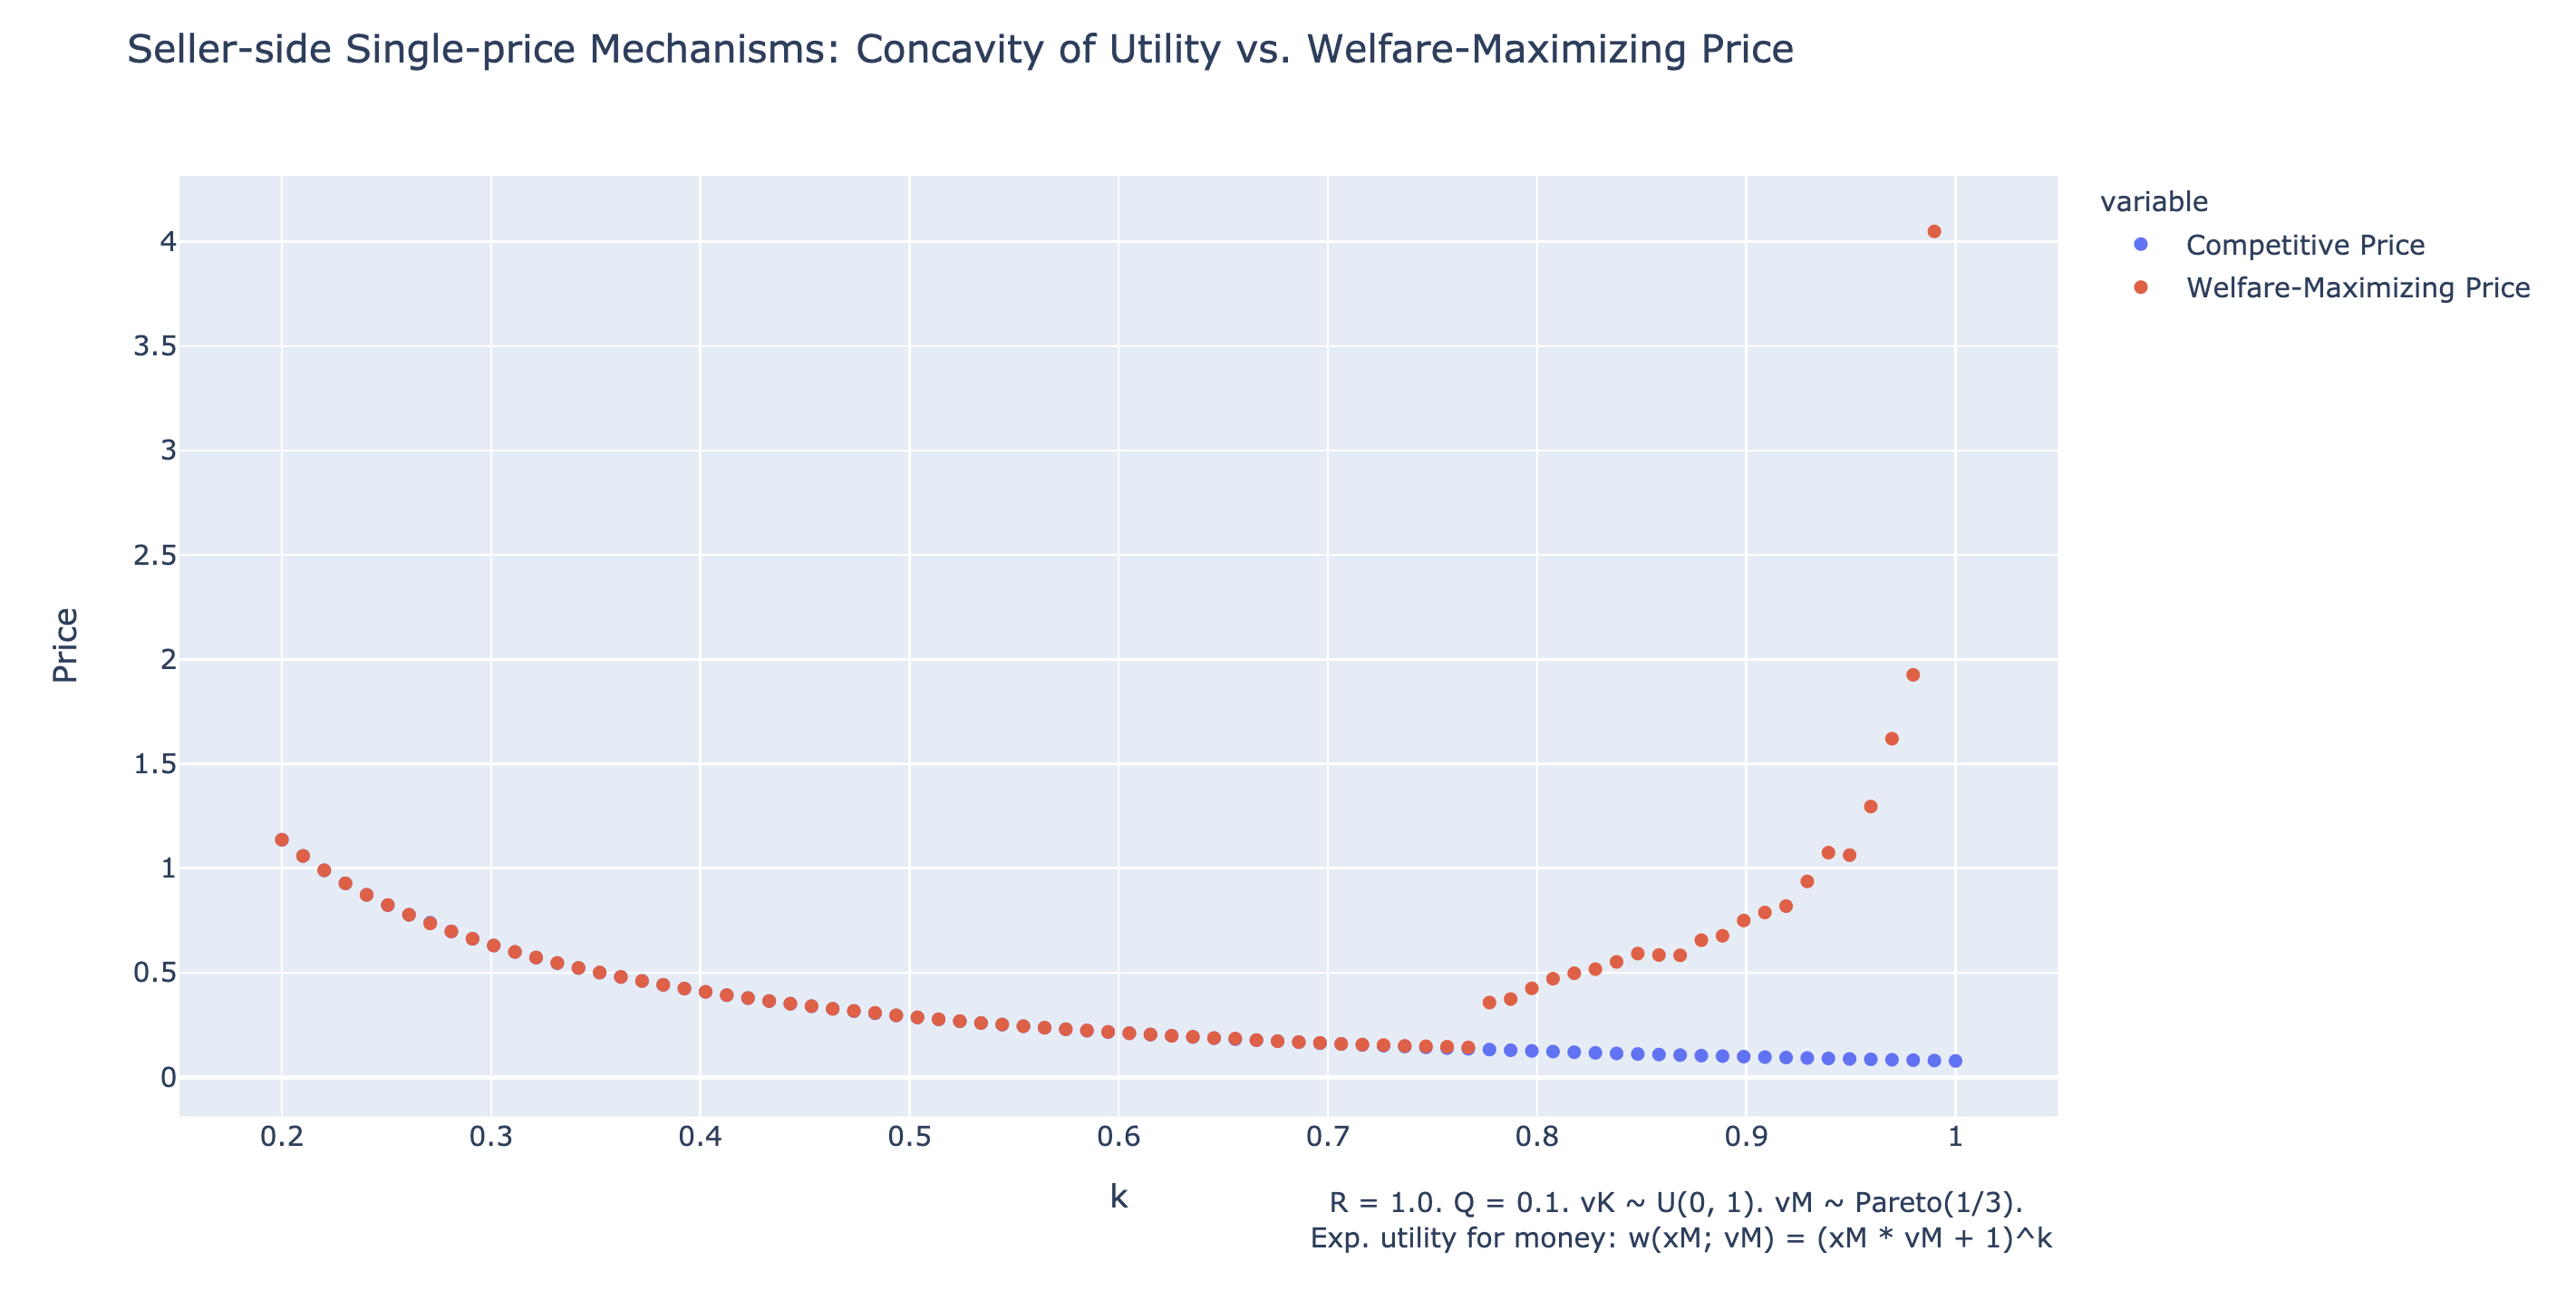
\includegraphics[width=\textwidth]{figures/k-vs-prices-inequality-high.png}
    \caption{Concavity of Utility (k) vs. Competitive Price and Welfare-Maximizing Price. High-inequality setting.}
\end{figure}

In both cases, we have only investigated two possible settings for the optimization problem, and we emphasize that it is an open question as to how much these results generalize to other settings.

\subsection{Conjectures}

Our work in the above sections suggest two corresponding analytic conjectures. First, our economic intuition in \ref{sec:economic-intuition} and our numerical simulations as in \ref{k-vs-prices-inequality-low} suggest that when the competitive price is optimal for the linear utility setting, it is also optimal in the concave-preference settings. Formally,

% Maybe: move these figures to sideways figures in appendix?
\begin{conj}
    \label{conj:competitive-price}
    % Add a segment on fixing R, Q, etc.?
    Suppose that when agent preferences for money are given by $w(x^M; v^M) = x^M v^M$, the optimal price is equal to the competitive price, so $p_S = p_S^C$. Holding all other parameters fixed, if we set agent preferences for money to any $w$ with $w$ concave, increasing in $v^M$ and satisfying $v'(0) = v^M$, then $p_S = p_S^C$ in the new setting.
\end{conj}

We suspect that Conjecture \ref{conj:competitive-price} can be solved by comparing the increased utility from higher lump-sum transfers to the decreased utility for higher sale prices of agents rationed in.

Our second conjecture corresponds to the numerical simulation result in \ref{k-vs-prices-inequality-high}.

\begin{conj}
    \label{conj:rationing-robust}
    % Add a segment on fixing R, Q, etc.?
    Consider the family of utility functions parametrized by $k$, with $w(x^M; v^M, k) = \frac{1}{k}(x^M v^M + 1)^k$. Suppose that when agent preferences for money are given by $w(x^M; v^M) = x^Ms v^M + 1$, the optimal mechanism involves rationing, so $p_S > p_S^C$. Then there exists some $\epsilon > 0$ such that for all $k \in (1-\epsilon, 1]$, rationing is optimal in the risk-averse setting with agent preferences for money given by $w(x^M; v^M, k)$.
\end{conj}

If true, this conjecture would suggest that the use of rationing as found in \cite{dworczak-2020} is reasonably robust to the presence of risk-aversion among agents. When rationing is optimal for linear preferences, it is also optimal for slightly concave preferences.

\section{Future Work}

More work is needed in three key directions: exactly characterizing the optimal mechanism for general concave preferences, characterizing optimality among all mechanisms, and extending this work to both sides of the market.

In the setting displayed in Figure \ref{k-vs-prices-inequality-high}, the welfare-maximizing price approaches the competitive price as preferences become more concave. However, more work is needed to verify exactly what the welfare-maximizing price is for various concave preferences. Alternatively, we could hope to find a threshold $k'$ for a given setting such that when preferences are sufficiently concave ($k < k'$), the competitive price must be optimal.

The second major area of extension is to generalize beyond single-price mechanisms to all possible mechanisms. We have covered only the first analysis of \cite{dworczak-2020}, which considers single-price mechanisms as a preliminary case to general mechanisms. It is possible to imagine that concave preferences lead to more complex optimal mechanisms, even though \cite{dworczak-2020} find that optimal mechanism generally take on a simple form. However, with general concave preferences, analytical approaches become particularly difficult. 

Finally, it remains to extend this work to a two-sided market, and solve joint optimality in the market. We have analyzed only the seller-side of the market, in which poorer sellers are those more likely to want to sell. In the buyer side, willingness to buy identifies the opposite, identifying buyers with a higher value for money. This could lead to qualitatively different behavior.

\section{Conclusion}

In this work, we analyzed the optimal single-price mechanism for maximizing total welfare in a setting where agents may have different marginal utilities for a good, and differing concave preferences for money. This setting is particularly relevant when designing price controls for labor markets. For example, when determining an appropriate minimum wage in a labor market, we should be concerned about wealth effects and agents' possible risk-aversion.

Our numerical simulation results validate this caustion, while also showing that the use of rationing can be robust to slight concavity in agents' preferences. We generalize the method of \cite{dworczak-2020} to formulate a welfare-maximization problem for general agent preferences for money. We then numerically simulate how the competitive price and welfare-maximizing price change as preferences become more concave.

Further work is needed to analytically solve for the optimal price under general preferences, to generalize to all mechanisms (not solely single-price mechanisms) and to extend our findings to a two-sided market. More broadly, the literature on redistribution through market design can benefit from a better understanding of how wealth effects shape optimal redistributive mechanisms. More precisely characterizing such mechanisms should yield implementable designs that are more robust to preferences in the wild.

% \section{Further Reading}
% \begin{itemize}
%     \item Scheuer, F. (2014): “Entrepreneurial taxation with endogenous entry,” American Economic Journal: Economic Policy, 6, 126–63.
            
%     \item Maybe: Saez, E., and Stantcheva, S. (2016). Generalized social marginal welfare weights for optimal tax theory. American Economic Review, 106(1), 24-45.
        
%     \item Condorelli 2013.
    
%     \item Kominers, S. and Teytelboym, A.: ``More Equal by Design: Economic Design Responses to Inequality". (Forthcoming book).

%     \item Work by Zi Yang Kang (or reach out to talk with him)
% \end{itemize}

% Some comments from meeting with Matt on 4/14:
% - There are generally two ways to generate relevant, interesting ideas in economic theory. You can start with theory and then find applications of that theory. Or you can start with applications and generate the theory from those applications.
% - Thinking about vaccines; what steps in the chain of vaccines are the most inequitable? Is it supply? Supply chains? Storage? Number of distribution sites? Savviness in accessing those sites?
% - Externalities are always an interesting, well-motivated question to explore: what happens if these groups have different externalities?
% - Could you model information and beliefs about vaccines? What about the network effects of increasing trust in vacccines?


% Comments from meeting with Mohammad on 4/22:
% - For risk-averse agents: does something more interesting happening than simply that rationing decreases? Does something happen beyond just less rationing? It could just be a threshold -- with concavity, a tiny bit might push you into a corner solution.
% - A divisible good could be interesting, but may not be tractable.
% - Another interesting idea is when investment before the mechanism is optimal. Perhaps rationing leads to missed or wasted investment.
% - Strong suggestion to start with simulations from the code. Try it out with slight concavity.

% Comments from meeting with Paul on 5/4:
% - Paul encouraged me to try a divisible item, even if it seemed (and Mohammad advised that it might be) intractable. Believe in yourself! Paul's first work, and Susan Athey's work under Paul, were both motivated by questions that their advisors felt they wouldn't be able to answer!
% - Understand Budish's metric of ex-post unfairness: random serial dictatorship is not always bad. Indeed, if there is only one good, it's in some way the only way to go. Budish's innovation is to bound unfairness when repeated by one good.

% Comments from meeting with Matt on 5/5:
% (2) Thesis Discussion
% - I've settled on a concrete idea. Mohammad's "Redistribution through Markets" (Dworczak 2020) paper considers agents with different marginal utilities for wealth, and determines optimal mechanisms in this situation. Some of these mechanisms involve rationing. However, agents' utilities are linear, hence the paper does not consider how agents' risk-aversions might affect the optimal mechanism. Indeed, if poorer individuals have low tolerance for uncertainty, the optimal mechanism may be very different than that derived in the original paper. A concrete extension is to attempt to derive optimal mechanisms when agents' preferences are risk-averse (slightly concave) and see when these mechanisms still involve rationing.
% - A few notes I clarified during the meeting: one example of a time when this decision comes into play is when, say, sellers have lower incomes than buyers, and so a price floor is typically imposed. (This is how Iran's kidney market operates, for example). With risk-averse preferences, you may not see this same price floor being an optimal mechanism. A second point of clarification: in the current model, agents have differing marginal utilities, but their utility functions are then linear in those marginal utilities.
% - I've talked about this with Mohammad, who suggested I begin with simulations of various mechanisms in an environment where agents have concave preferences. He even sent me over some of his existing simulation code! I think this is a great starting point.
% - We also talked about advisors; Matt suggested Mohammad as the best possible advisor (which stands to reason). He suggested that if Mohammad couldn't advise, one of the other theorists in the department, like Paul or Ilya, would probably be more equipped to advise this thesis than Matt. It's allso lovely to have a group of people who I continue talking to about the thesis.
% - Some ideas we discussed:
% 	- I can reframe this more broadly as "why is the uncertainty associated with rationing undesirable?" These arguments might also find some inspiration in early economic philosophers (Adam Smith, perhaps Hayek too). In general, the arbitrariness of inequality imposed within a group by rationing feels undesirable. Maybe there's some interesting "veil of ignorance" type arguments here.
% 	- One example is healthcare queueing costs -- the uncertainty of not knowing whether you'll be waiting one month or ten months for a surgery can be very harmful.
% 	- Another example of where ex-post fairness matters: in Eric Budish's paper on combinatorial allocations, one allocation that is ex-ante fair is a random serial dictatorship. It is definitely not ex-post fair. This is not what most of us would consider optimal!
% - A few ideas that I had afterwards:
% 	- I can sharpen a concrete counterexample of when the mechanism from Dworczak (2020) produces an ex-ante optimal mechanism, but seems unpalatable to observers because of wide ex-post inequalities that it imposes.
% 	- Another idea: one reason this idea attracted me is that poor agents might be more likely to actually be risk averse (less cash liquidity, tolerance for income shocks, etc.). What if this is reflected in poorer agents having more risk-averse preferences?)


% Remove or comment out the next two lines if you are not using bibtex.
\bibliographystyle{aea}
\bibliography{inequality-design}

% The appendix command is issued once, prior to all appendices, if any.

\end{document}

